% created on 16/11/2020
% @author : ebazan

\chapter{Landing Target Description}\label{ch:target_description}
In this appendix we describe the landing target design process used in chapter \ref{ch:landing_target_detection} for detection and identification in the autonomous landing task. The landing target is formed by a set of black and white circles (see figure \ref{fig:target_description}) that generate contours when stacked. Two of the circles ($\diameter_{9}$ and $\diameter_{10}$) have a constant diameter and form the ring that defines the target. The black circle ($\diameter_{11}$) is an orientation reference and has the same diameter as the smallest circle, $\diameter_{11}=\diameter_{1}$. The other circles $\diameter_{1}, \ldots, \diameter_{8}$ are coding circles.


\begin{figure}[!ht]
\centering
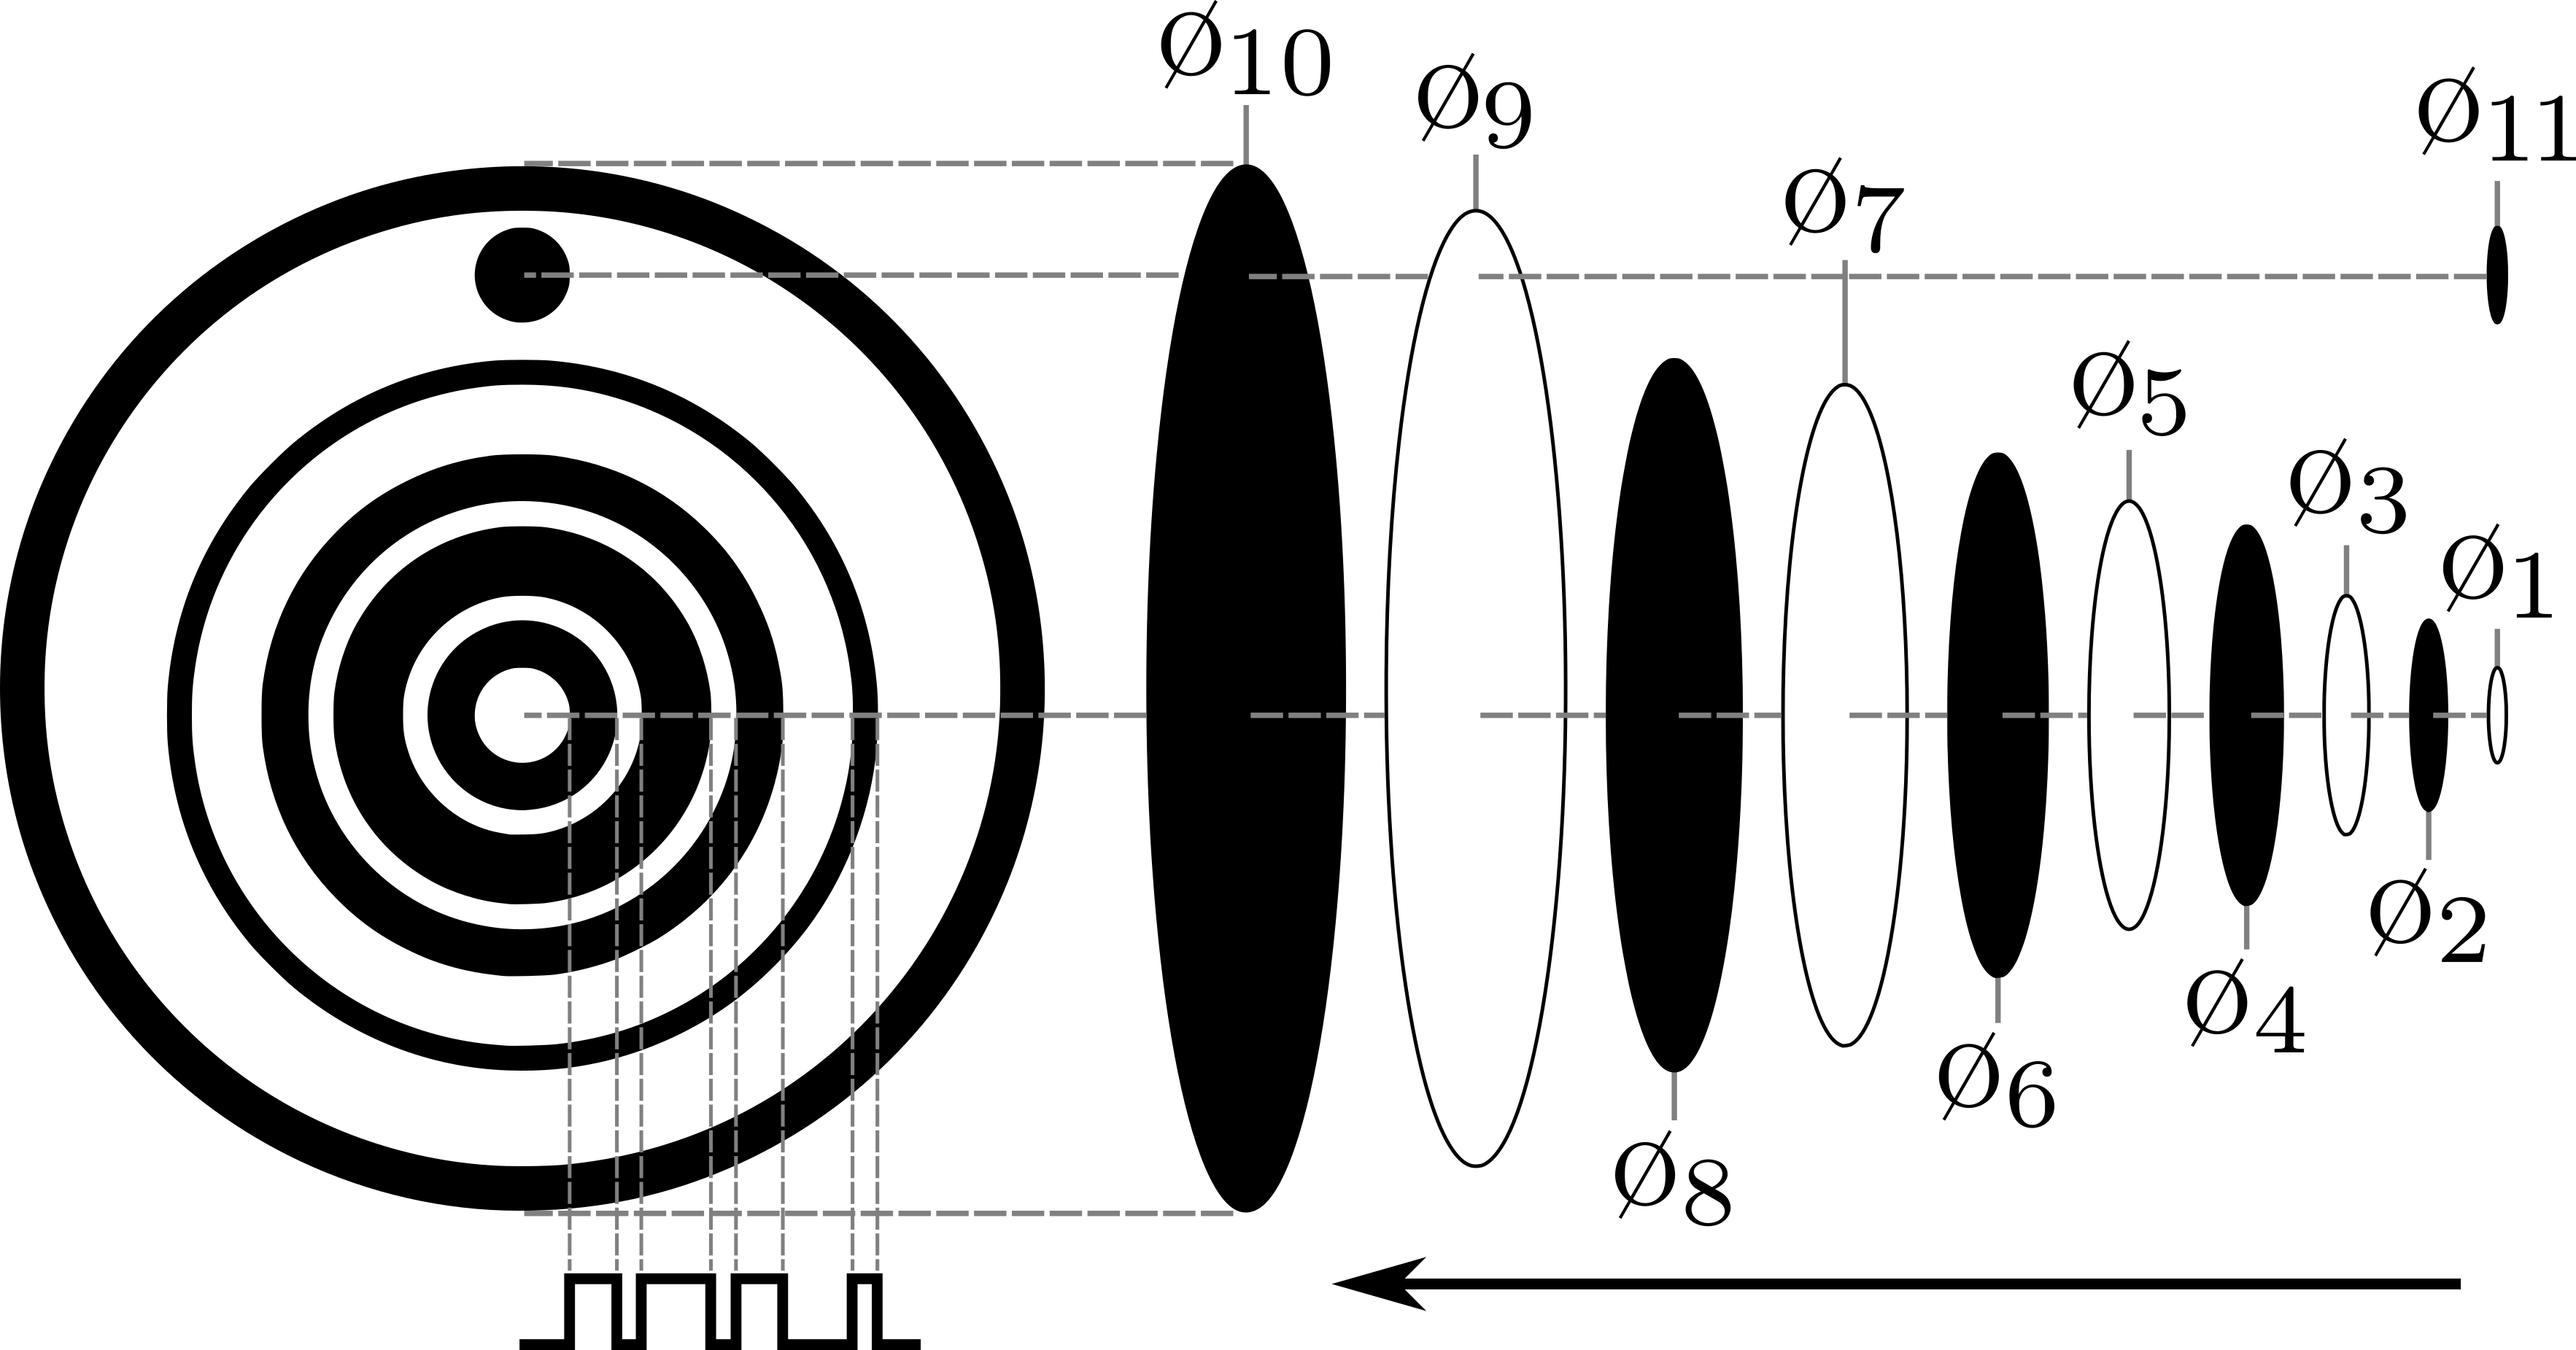
\includegraphics[width=\textwidth]{target_description}
\caption{Landing target design and description}
\label{fig:target_description}
\end{figure}

\section{Landing Target ID Encoding}
Let $\varnothing=\left( \diameter_{1}, \diameter_{2},\ldots,\diameter_{n}\right) $ denote the nominal diameters of the coding circles. We can set the nominal diameters, e.g., $\diameter_{i}=\frac{i}{n}\diameter_{n}$ for a target without the encoding capability. To encode a number in the target form, we modify the nominal diameters $\varnothing$ to obtain $\varnothing'=\left( \diameter_{1}', \diameter_{2}',\ldots,\diameter_{n}'\right) $ by adding/subtracting a positive constant $\Delta h$
\begin{equation}
\diameter_{i}'=
\begin{cases}
  \diameter_{i}+\Delta h, & \text{if } w_{i}=1 \\
  \diameter_{i}- \Delta h, & \text{otherwise }
\end{cases}
\end{equation}
and obtain a binary message  $W=[w_{1}, \dots,w_{n}]$. The message $W$ is protected from errors by error-correction Hamming code  \citep{Hamming:BSTJ:1950}. It provides a set of different codewords $W= D\times M$ of size $n=k+m$, where $D$ is useful data, $ M=[I_{k}\mid 1-I_{k}]$ the generator matrix and $I_{k}$ is the $k\times k$ the identity matrix. The data vector $D$ comes from the decimal to binary conversion of the landing target ID number. For the experiments showed in chapter , we have created landing targets with $n=8$ coding circles allowing to have four rings and $8$ contours $\diameter_{1}, \ldots, \diameter_{8}$. This allows us to use the extended $[n,k]$ Hamming code with $k=4$ data bits and $m=4$ parity bits to generate $2^{4}=16$ landing targets. The set of landing targets generated using this configuration can be seen in the figure \ref{fig:landing_target_database}.

\section{Landing Target ID Decoding.}
After the clustering stage of section \ref{subsec:clustering}, we rank by size the ellipses' major axes $\alpha_i$ by size and normalize them w.r.t. the largest value $\alpha_{10}$ to obtain %$A=(\alpha_{1}, \ldots, \alpha_{10})$  \raisebox{1mm}{$\diameter_{10}$}$/$\raisebox{-1mm}{$\alpha_{10}$}.
$\vec{\alpha}=  \frac{\diameter_{10}}{\alpha_{10}} (\alpha_{1}, \ldots, \alpha_{10})$

We compare the received and normalized axis $\vec{\alpha}$ with the nominal diameters of the coding circles $\varnothing$ and transform them into a binary vector $\widehat{W}$;
\begin{equation}
\widehat{W}=
\begin{cases}
  1, & \text{if } \alpha_{i}-\diameter_{i} > 0 \\
  0, & \text{otherwise}
\end{cases} \enspace \forall i=1,\ldots, n
\end{equation}
The Hamming syndrome vector $S=\widehat{W}\times H^{T}$ (with $H=[1-I_{k}\mid I_{k}]$ as the parity-check matrix) indicates whether an error has occurred. The syndrome is a null vector $S=0$ when no error has occurred, otherwise, $S\neq 0$ and $\widehat{W}=W+E$. The element $e_{i}=0$ of the error vector $E=H^{T}-S$ indicates an error at the position $i$. The $[8,4]$ Hamming code can find up to two erroneous bits and correct one. Once the algorithm corrects the error (if there is), the vector $\widehat{W}$ is decoded by using the modulo 2 of the product $\widehat{D}=\widehat{W}\times M^{T}$. 

\begin{figure}[!ht]
	\centering
	\begin{subfigure}[b]{0.23\textwidth}
		\centering
		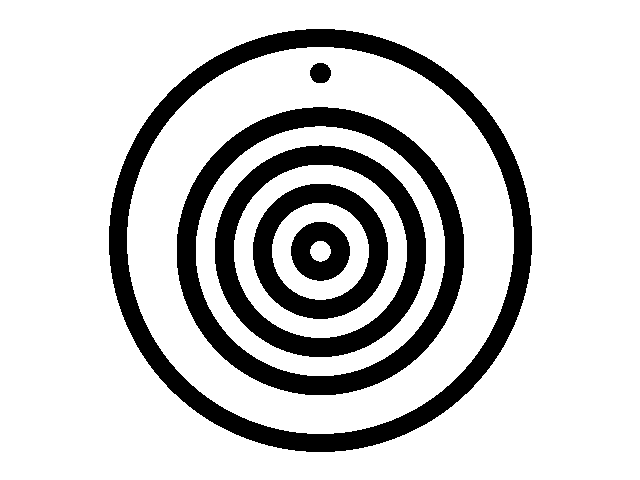
\includegraphics[trim={3.5cm 0 3.5cm 0}, clip, width=\textwidth]{normal_target0}
	    \caption{Target ID 0}
	\end{subfigure}
	~ %add desired spacing between images, e. g. ~, \quad, \qquad, \hfill etc. 
    %(or a blank line to force the subfigure onto a new line)
    \begin{subfigure}[b]{0.23\textwidth}
		\centering
		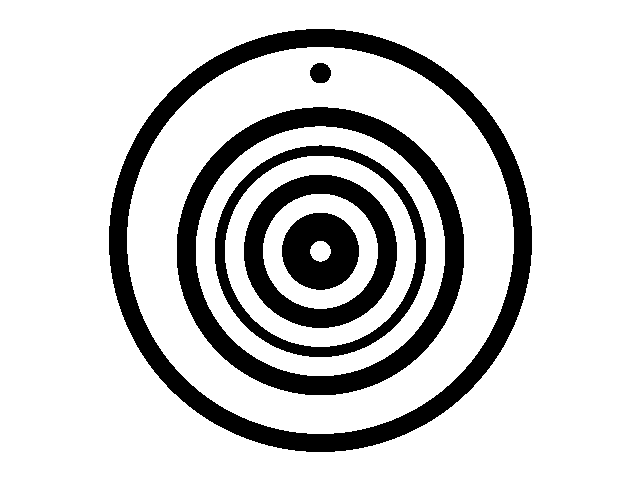
\includegraphics[trim={3.5cm 0 3.5cm 0}, clip, width=\textwidth]{normal_target1}
		\caption{Target ID 1}	
	\end{subfigure}
    ~ %add desired spacing between images, e. g. ~, \quad, \qquad, \hfill etc. 
    %(or a blank line to force the subfigure onto a new line)
    \begin{subfigure}[b]{0.23\textwidth}
		\centering
		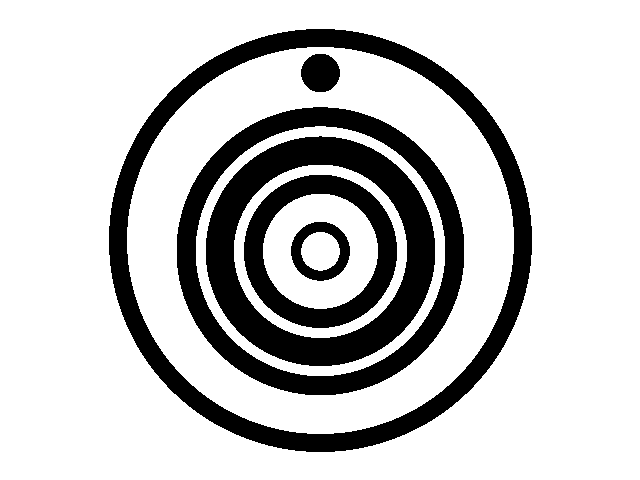
\includegraphics[trim={3.5cm 0 3.5cm 0}, clip, width=\textwidth]{normal_target2}	
		\caption{Target ID 2}
	\end{subfigure}
	~ %add desired spacing between images, e. g. ~, \quad, \qquad, \hfill etc. 
    %(or a blank line to force the subfigure onto a new line)
    \begin{subfigure}[b]{0.23\textwidth}
		\centering
		
\includegraphics[trim={3.5cm 0 3.5cm 0}, clip, width=\textwidth]{normal_target3}	
		\caption{Target ID 3}
	\end{subfigure} \\[2ex]
    
    
    \begin{subfigure}[b]{0.23\textwidth}
		\centering
		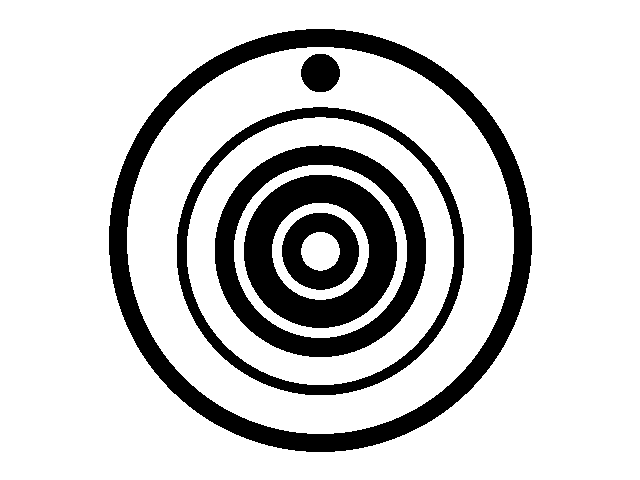
\includegraphics[trim={3.5cm 0 3.5cm 0}, clip, width=\textwidth]{normal_target4}	
		\caption{Target ID 4}
	\end{subfigure}
    ~ %add desired spacing between images, e. g. ~, \quad, \qquad, \hfill etc. 
    %(or a blank line to force the subfigure onto a new line)
    \begin{subfigure}[b]{0.23\textwidth}
		\centering
		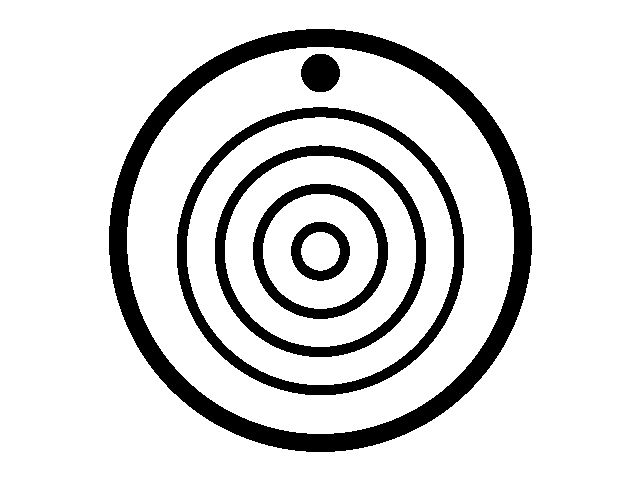
\includegraphics[trim={3.5cm 0 3.5cm 0}, clip, width=\textwidth]{normal_target5}	
		\caption{Target ID 5}
	\end{subfigure}
    ~ %add desired spacing between images, e. g. ~, \quad, \qquad, \hfill etc. 
    %(or a blank line to force the subfigure onto a new line)
    \begin{subfigure}[b]{0.23\textwidth}
		\centering
		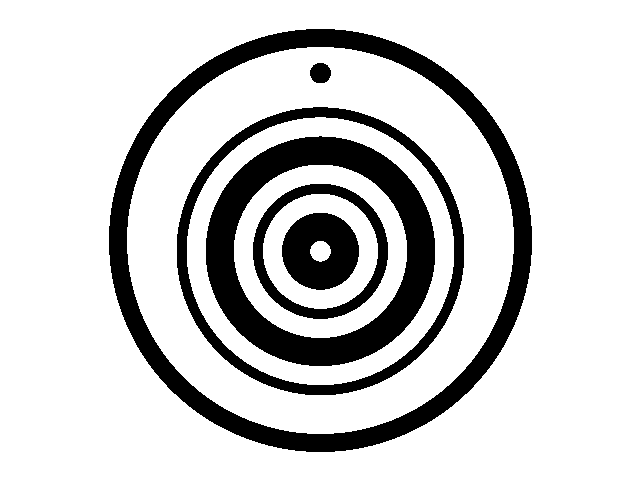
\includegraphics[trim={3.5cm 0 3.5cm 0}, clip, width=\textwidth]{normal_target6}	
		\caption{Target ID 6}
	\end{subfigure}
	~ %add desired spacing between images, e. g. ~, \quad, \qquad, \hfill etc. 
    %(or a blank line to force the subfigure onto a new line)         
    \begin{subfigure}[b]{0.23\textwidth}
		\centering
		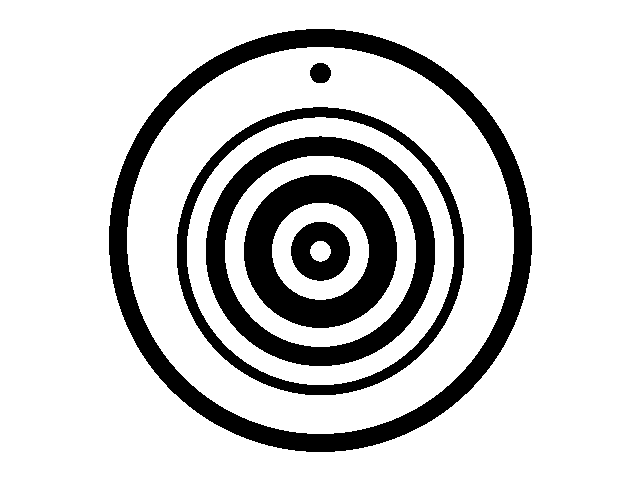
\includegraphics[trim={3.5cm 0 3.5cm 0}, clip, width=\textwidth]{normal_target7}	
		\caption{Target ID 7}
	\end{subfigure}  \\[2ex]
	
	
    \begin{subfigure}[b]{0.23\textwidth}
		\centering
		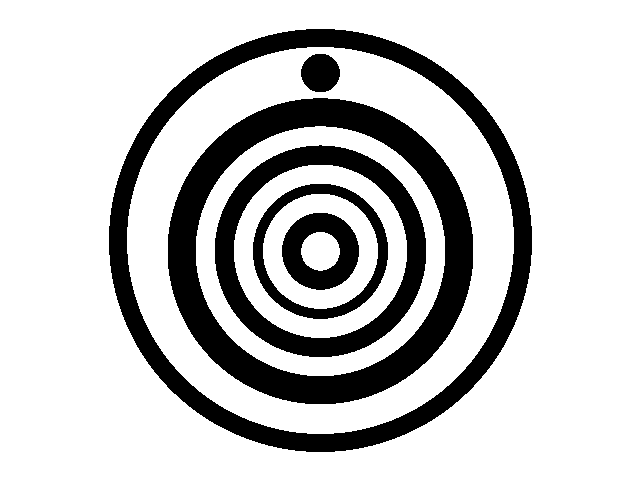
\includegraphics[trim={3.5cm 0 3.5cm 0}, clip, width=\textwidth]{normal_target8}	
		\caption{Target ID 8}
	\end{subfigure}
    ~ %add desired spacing between images, e. g. ~, \quad, \qquad, \hfill etc. 
    %(or a blank line to force the subfigure onto a new line)
    \begin{subfigure}[b]{0.23\textwidth}
		\centering
		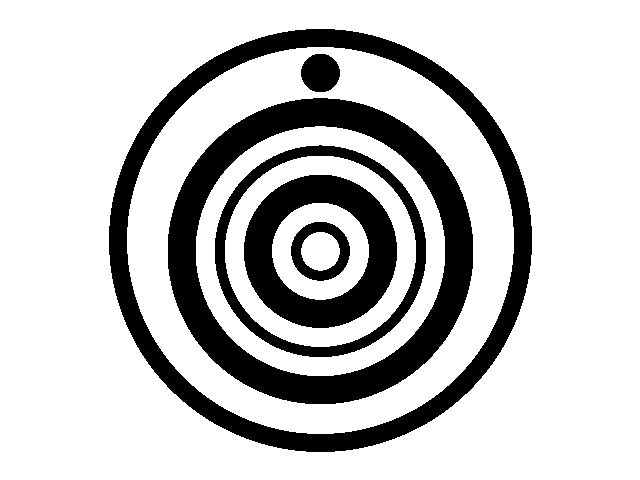
\includegraphics[trim={3.5cm 0 3.5cm 0}, clip, width=\textwidth]{normal_target9}	
		\caption{Target ID 9}
	\end{subfigure}
	~ %add desired spacing between images, e. g. ~, \quad, \qquad, \hfill etc. 
    %(or a blank line to force the subfigure onto a new line)
    \begin{subfigure}[b]{0.23\textwidth}
		\centering
		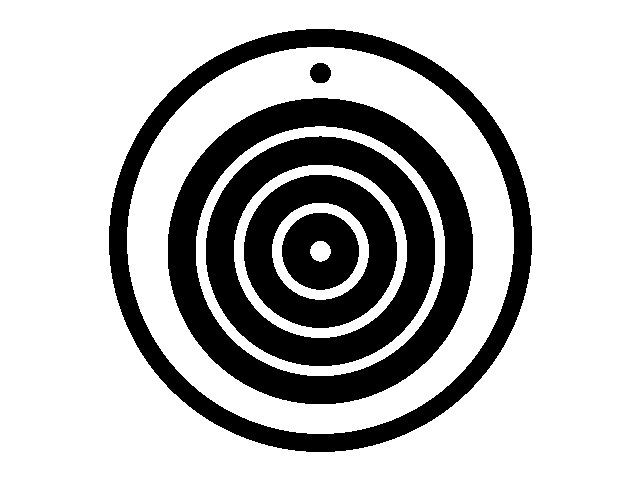
\includegraphics[trim={3.5cm 0 3.5cm 0}, clip, width=\textwidth]{normal_target10}	
		\caption{Target ID 10}
	\end{subfigure}
	~ %add desired spacing between images, e. g. ~, \quad, \qquad, \hfill etc. 
    %(or a blank line to force the subfigure onto a new line) 
    \begin{subfigure}[b]{0.23\textwidth}
		\centering
		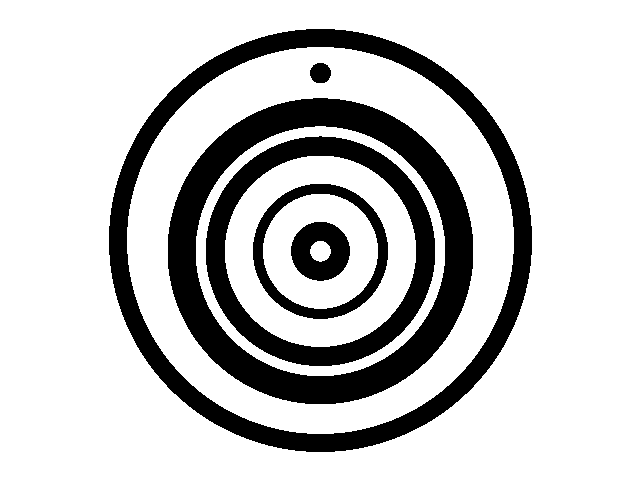
\includegraphics[trim={3.5cm 0 3.5cm 0}, clip, width=\textwidth]{normal_target11}	
		\caption{Target ID 11}
	\end{subfigure} \\[2ex]    
    
    
    \begin{subfigure}[b]{0.23\textwidth}
		\centering
		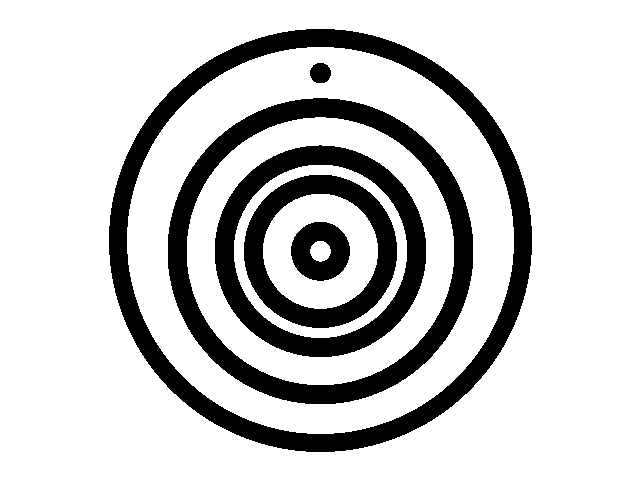
\includegraphics[trim={3.5cm 0 3.5cm 0}, clip, width=\textwidth]{normal_target12}	
		\caption{Target ID 12}
	\end{subfigure}
    ~ %add desired spacing between images, e. g. ~, \quad, \qquad, \hfill etc. 
    %(or a blank line to force the subfigure onto a new line)
    \begin{subfigure}[b]{0.23\textwidth}
		\centering
		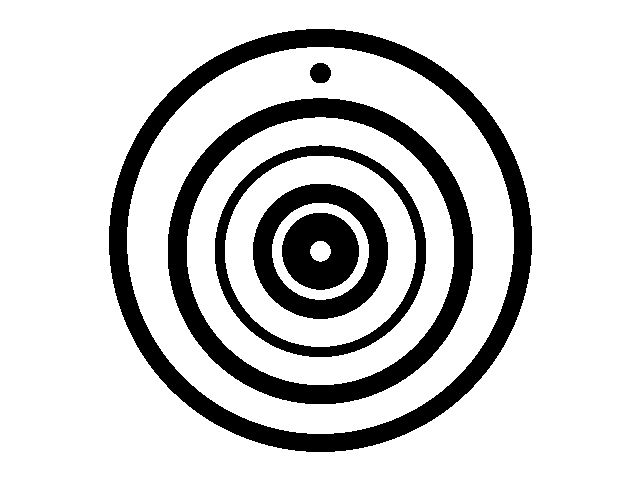
\includegraphics[trim={3.5cm 0 3.5cm 0}, clip, width=\textwidth]{normal_target13}	
		\caption{Target ID 13}
	\end{subfigure} 
     ~ %add desired spacing between images, e. g. ~, \quad, \qquad, \hfill etc. 
    %(or a blank line to force the subfigure onto a new line)    
    \begin{subfigure}[b]{0.23\textwidth}
		\centering
		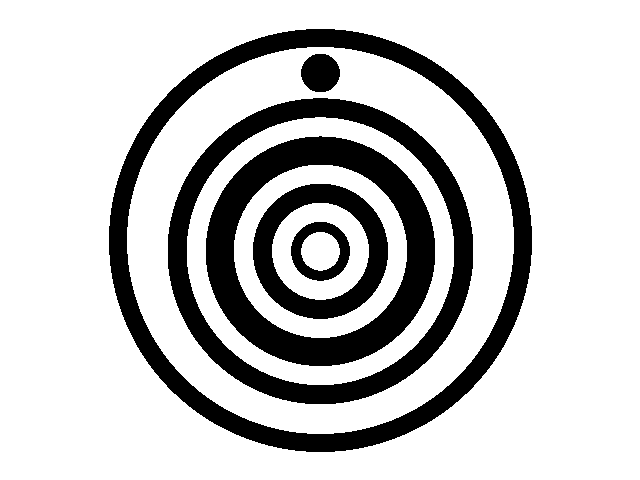
\includegraphics[trim={3.5cm 0 3.5cm 0}, clip, width=\textwidth]{normal_target14}	
		\caption{Target ID 14}
	\end{subfigure}
	~ %add desired spacing between images, e. g. ~, \quad, \qquad, \hfill etc. 
    %(or a blank line to force the subfigure onto a new line)
    \begin{subfigure}[b]{0.23\textwidth}
		\centering
		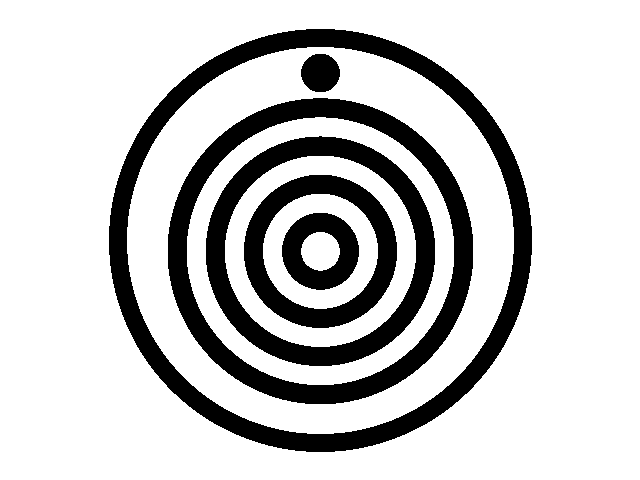
\includegraphics[trim={3.5cm 0 3.5cm 0}, clip, width=\textwidth]{normal_target15}	
		\caption{Target ID 15}
	\end{subfigure}    
		
    \caption{Landing target database generated with error-correction Hamming code.}
    \label{fig:landing_target_database}
\end{figure}
